\subsection{Генераторы данных}

Для проведения вычислительных экспериментов в рамках данной работы была разработана система генерации тестовых данных, включающая два основных компонента:
\begin{itemize}
    \item генератор графов в формате METIS с дополнительной геометрической информацией;
    \item генератор запросов поиска пути с моделированием различных паттернов нагрузки.
\end{itemize}

Данные компоненты позволяют формировать контролируемую экспериментальную среду, в которой можно исследовать влияние структуры графа и характера запросов на эффективность алгоритмов распределения данных.

\subsubsection{Генерация графа}

Граф представляется в формате METIS, состоящем из списка смежности. Первая строка файла содержит два числа:
\begin{equation*}
    N, M,
\end{equation*}
где $N$ --- количество вершин графа, $M$ --- количество рёбер.

Каждая последующая строка $i$ описывает множество вершин, смежных с вершиной $v_i$.

Дополнительно для каждой вершины генерируются координаты в двумерном пространстве:
\begin{equation*}
    v_i \rightarrow (x_i, y_i), \quad x_i, y_i \in [0, L],
\end{equation*}
где $L$ задаёт размер области генерации.

Генерация графа выполняется следующим образом:

\begin{enumerate}
    \item задаётся количество вершин $N$ и средняя степень вершины $d$;
    
    \item для каждой вершины генерируются координаты $(x_i, y_i)$ с использованием равномерного распределения на квадрате $[0, L] \times [0, L]$;

    \item инициализируется список смежности $G = (V, E)$;

    \item для обеспечения связности графа добавляются рёбра вида:
    \begin{equation*}
        (v_i, v_{i+1}), \quad i = 1 \dots N-1.
    \end{equation*}

    \item далее добавляются случайные рёбра до достижения требуемого количества:
    \begin{equation*}
        M \approx \frac{N \cdot d}{2}.
    \end{equation*}

    При добавлении рёбер исключаются:
    \begin{itemize}
        \item петли $(v_i, v_i)$;
        \item дубликаты рёбер.
    \end{itemize}

    \item сформированный граф записывается в METIS-формат.
\end{enumerate}

Таким образом, получаем граф, обладающий одновременно:
\begin{itemize}
    \item топологической структурой (через список смежности);
    \item геометрической локальностью (через координаты вершин).
\end{itemize}

\textit{Входной формат графа}

Основной входной формат графа соответствует стандарту METIS и используется для задания структуры графа в виде списка смежности.

Файл графа состоит из двух частей:
\begin{itemize}
    \item заголовок:
    \begin{equation*}
        N \quad M,
    \end{equation*}
    где $N$ --- количество вершин, $M$ --- количество рёбер;

    \item список смежности: каждая последующая строка $i$ содержит индексы вершин, смежных с вершиной $v_i$.
\end{itemize}

Индексация вершин начинается с 1. Для неориентированного графа каждое ребро представляется дважды в списках смежности.

Данный формат используется основным алгоритмическим ядром системы для построения распределённого графа и выполнения операций поиска пути.

Дополнительно к структуре графа формируется файл координат вершин, используемый для моделирования пространственной локальности.

Формат файла представляет собой последовательность строк:
\begin{equation*}
    x_i \quad y_i,
\end{equation*}
где $x_i$ и $y_i$ --- координаты вершины $v_i$ в двумерном пространстве.

Следовательно, файл координат должен отвечать следующим требованиям:
\begin{itemize}
    \item каждая строка соответствует одной вершине;
    \item порядок строк совпадает с порядком вершин в METIS-файле;
    \item значения координат задаются в вещественном формате.
\end{itemize}

Данный файл используется генератором запросов для построения локальных и кластерных паттернов нагрузки.

То есть, например, файлы на листингах \ref{gen-lst:graph} и \ref{gen-lst:coords} представляют граф на рисунке \ref{gen-fig:graph}.

\begin{lstlisting}[caption=Пример файла графа, label=gen-lst:graph]
4 5
2 3 4
1 4
1 4
1 2 3
\end{lstlisting}

\begin{lstlisting}[caption=Пример файла координат, label=gen-lst:coords]
0 0
1 0
0 1
1 1
\end{lstlisting}

\begin{figure}[h]
    \centering
    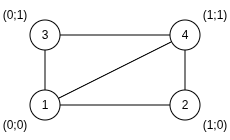
\includegraphics[width=.5\textwidth]{extras/technological_part/graph_example.png}
    \caption{Пример выходного графа, представленного файлами из листингов \ref{gen-lst:graph} и \ref{gen-lst:coords} }
    \label{gen-fig:graph}
\end{figure}

\subsubsection{Генерация запросов}

Генератор запросов формирует набор запросов поиска пути между вершинами графа:
\begin{equation*}
    q = (v_s, v_t),
\end{equation*}
где $v_s$ --- начальная вершина, $v_t$ --- конечная вершина.

Каждый запрос относится к одному из нескольких типов, что позволяет моделировать различные сценарии нагрузки.

\textit{Типы запросов}

1. Случайные запросы

С вероятностью $p_1 = 0.4$ выбираются две случайные вершины:
\begin{equation*}
    v_s, v_t \sim U(1, N).
\end{equation*}

Данный тип нагрузки моделирует равномерное обращение ко всем частям графа.

2. Локальные запросы

С вероятностью $p_2 = 0.3$ используется пространственная локальность.

Выбирается центральная вершина $v_c$, после чего формируется множество:
\begin{equation*}
    S = \{ v_i \mid d(v_i, v_c) \le R \},
\end{equation*}
где расстояние определяется как евклидово:
\begin{equation*}
    d(v_i, v_j) = \sqrt{(x_i - x_j)^2 + (y_i - y_j)^2}.
\end{equation*}

Конечная вершина выбирается из множества $S$.

3. Запросы через хабы

С вероятностью $p_3 = 0.2$ используются вершины-хабы.

Хабы выбираются заранее:
\begin{equation*}
    |H| = \frac{N}{100}.
\end{equation*}

Формирование запроса:
\begin{itemize}
    \item либо $v_s \in H$, $v_t \sim U(1, N)$;
    \item либо $v_t \in H$, $v_s \sim U(1, N)$.
\end{itemize}

4. Кластерные запросы

С вероятностью $p_4 = 0.1$ формируются кластерные запросы.

Выбирается центр кластера $v_c$ и радиус $R_c > R$, после чего обе вершины выбираются из множества:
\begin{equation*}
    S_c = \{ v_i \mid d(v_i, v_c) \le R_c \}.
\end{equation*}

5. Графовые локальные запросы

Дополнительно могут использоваться запросы, основанные на структуре графа.

Выбирается вершина $v_s$, после чего вершина $v_t$ выбирается из её окрестности:
\begin{equation*}
    v_t \in BFS(v_s, k),
\end{equation*}
где $k$ --- глубина обхода.

\textit{Общий алгоритм генерации}

Для каждого запроса выполняется следующий набор действий:
\begin{enumerate}
    \item генерируется случайное число $r \in [0,1]$;
    \item в зависимости от диапазона выбирается тип запроса:
    \begin{itemize}
        \item $r < 0.4$ --- случайный;
        \item $0.4 \le r < 0.7$ --- локальный;
        \item $0.7 \le r < 0.9$ --- через хаб;
        \item $0.9 \le r < 1.0$ --- кластерный.
    \end{itemize}
    \item формируется пара вершин $(v_s, v_t)$;
    \item запрос записывается в выходной файл.
\end{enumerate}

\textit{Формат файла запросов}

Результатом работы генератора запросов является файл, содержащий последовательность запросов поиска пути.

Общий формат:
\begin{equation*}
    type \quad v_s \quad v_t, 
\end{equation*}

где:
\begin{itemize}
    \item $type$ --- тип запроса (RANDOM, LOCAL, HUB, CLUSTER, GRAPH\_LOCAL);
    \item $v_s$ --- начальная вершина;
    \item $v_t$ --- конечная вершина.
\end{itemize}

Первая строка файла содержит общее количество запросов $Q$.

\textit{Результат}

Предложенная система генерации тестовых данных позволяет моделировать:
\begin{itemize}
    \item равномерную нагрузку;
    \item локально-структурированные обращения;
    \item кластерные паттерны;
    \item обращения через высокостепенные вершины.
\end{itemize}

Благодаря этому достигается реалистичная имитация поведения распределённых графовых систем и создаются условия для объективного сравнения алгоритмов потокового распределения и оптимизации разбиения графа.
